\xchapter{Análise do ciclo de vida dos projetos}
{Este capítulo apresenta ...}

A seção \ref{sec:study1:intro} apresenta ...
seção \ref{sec:study1:definition} ...
seção \ref{sec:study1:operation} ...

% Introduction
% Background
% Experimental Setup (hipoteses / design)
% Results (data analysis)
% Discussion
% Threats to validity
% Conclusions

\section{Introdução e Motivação} \label{sec:study1:intro}

%TROUXE da INTRODUCAO e revisei. PRECISA DE CITACOES.
O software desenvolvido na academia sofre de {\it ``dysfunctional chaotic churn''} [CITAR].
Na prática, isso significa que há muitos projetos com características e funcionalidades parecidas, 
com poucos usuários, com ciclos de vida curtos, e encerrados quando o financiamento inicial termina,
bem como, comunidades desconectadas e paralelas, incompatibilidades entre projetos em um mesmo domínio, 
e tentativas aparentemente não coordenadas de ``reiniciar'' tudo ({\it re-boots}).

\textbf{O caso do Analizo.}  Descrever uma situação em que software acadêmico foi necessário
para apoiar pesquisa. egypt, etc. analizo, comunidade, usp, etc.
menções ...

Analizo \cite{Terceiro2010Analizo} é um conjunto de ferramentas para análise de código-fonte e
visualização com suporte a múltiplas linguagens de programação, software livre,
extensível e capaz de lidar com código-fonte não mais compilável. A capacidade
de lidar com código-fonte não mais compilável permite analisar código-fonte
com erros de sintaxe, com referências a bibliotecas não mais disponíveis, ou
que usem bibliotecas com mudanças de API.

Analizo tem sido extensivamente usado por nosso grupo de pesquisa em diversos
estudos.
\cite{Amaral2009} usou o grafo de dependencia gerado pelo Analizo para
  gerar uma matriz de evolução em um estudo de caso com o projeto VLC.
\cite{Costa2009} fez uma comparação entre diferentes estratégias para
  extração de informação de dependencias entre módulos do código-fonte,
  resultando no desenvolvimento do Doxyparse - o extrator baseado no Doxygen do
  Analizo.
\cite{Terceiro2009} usou métricas em um estudo exploratório sobre a
  evolução da complexidade estrutural em projetos de software livre escritos em
  C.
\cite{Morais2009} usou a ferramenta de métricas do Analizo como backend
  para o Kalibro, um software para avaliação e observação de métricas de código-fonte.
\cite{Terceiro2010} usou o processamento de histórico de métricas para
  realizar um estudo exploratório sobre a evolução da complexidade estrutural em
  7 projetos de servidor web de diferentes tamanhos.
\cite{Meirelles2010} usou o processamento em lote do Analizo para
  processas o código-fonte de mais de 6000 projetos de software livre do
  repositório Sourceforge.net.
\cite{Meirelles2011} usou o Analizo em um estudo sobre impacto de
  métricas de código-fonte na atratividade de projetos de softwares livres.
\cite{Terceiro2012Understanding} usou o Analizo para investigar fatores
  que influenciam na evolução da complexidade estrutural em projetos de software
  livres.
\cite{Silva2012} usou o Analizo para minerar 16000 revisões de
  repositórios de projetos de software para investigar o potencial de uma nova
  métrica chamada Lack of Concern-based Cohesion.

% \cite{Ronaldo2015}

% \cite{Mateus2017}

A maioria destes trabalhos contribuíram com melhorias para o Analizo, fazendo
dele uma ferramenta bastante apropriada para pesquisas envolvendo análise de código-fonte,
sendo útil tanto para pesquisadores trabalhando com análise de código-fonte
quanto para profissionais que precisam analisar seus projetos em busca de
potenciais problemas ou melhorias.

Analizo é software livre, distribuído sob a licença GNU General Public License
versão 3. Seu código-fonte, bem como pacotes binários, manuais e tutoriais
podem ser obtidos em \url{http://www.analizo.org}. Todas as ferramentas são
auto-documentadas e podem ser consultadas como páginas de manual UNIX. Analizo
é escrito em Perl, sua última versão 1.19.1 lançada em 01 de Setembro de 2016
foi a versão utilizada neste estudo.


% TRAZER/USAR o termo ecossistema de software aqui?
% Creio que o termo ```projeto'' atende ... a discutir.
% Como usar outros elementos do ecossistema neste capitulo, por exemplo, atores?
% Sustentabilidade técnica para a ciência de um modo geral?  ou sócio-técnica?


\section{Definição} \label{sec:study1:definition}

% Por que o estudo será realizado?

O que sabemos sobre a sustentabilidade técnica de projetos de software acadêmico publicados em conferências
de Engenharia de Software? Como estes projetos são mencionados na literatura acadêmica?   
Colocar QUESTAO SOBRE COLABORACAO.


\subsection{Definição do Objetivo}

\begin{description}
\item{\bf Objeto de estudo.} 
O objeto de estudo são projetos de software acadêmico de análise estática e sua sustentabilidade técnica.

\item{\bf Propósito.} 
O propósito deste estudo é caracterizar a sustentabilidade técnica de cada software acadêmico de análise estática,
trazendo informações que permitam ...

\item{\bf Perspectiva.} 
A perspectiva considerada é a de cientistas e pesquisadores, isto é, 
o cientista ou pesquisador gostaria de conhecer ecossistemas de software acadêmico de análise estática
em termos de sua sustentabilidade técnica. 
Além disso, pessoas da indústria podem estar interessadas em conhecer
software acadêmico de análise estática para financiá-lo.

\item{\bf Foco de qualidade.} 
O principal aspecto de qualidade estudado é a sustentabilidade sócio-técnica,
com destaque para três aspectos: transparência, complexidade e adoção.
%, A, B, C ... EXPLICAR A, B, C.


Q1 é demográfica?
Transparência: aberto? disponível? transparente?  Funciona? Ver Q2.
Adoção: ver Q4.
Q3? Parece que há duas questões em uma. Você vai olhar todas as versões para tratar da visibilidade??
A outra questão tem a ver sobre como referenciar software em artigos científicos?
Complexidade: qualidade do código.  Estudo 2.

\item{\bf Contexto.} 
O estudo foi conduzido com projetos de software acadêmico de análise estática
publicados nas conferências ASE e SCAM.
\end{description}

\subsection{Sumário da Definição}

%% QUERO DISCUTIR SE SUSTENTABILIDADE JA EH MENCIONADA OU NAO no Object of Study

%% GQM template

Analisar a \textit{software acadêmico de análise estática e sua sustentabilidade técnica} % object of study
com o propósito de \textit{caracterizar}  % purpose  % era medir e avaliar - coloquei 'caracterizar' 
com respeito a \textit{disponibilidade de código, números de citações e complexidade estrutural (manutenibilidade)}  % quality focus
na perspectiva do \textit{pesquisador} e do \textit{cientista}% perspective
no contexto de \textit{software acadêmico de análise estática publicado nas conferências ASE e SCAM 
e referenciado por artigos publicados nas bases da ACM e IEEE}. % context
%


\subsection{Questões de Pesquisa}

Neste estudo as seguintes questões de pesquisa, a respeito do ecossistema de
software acadêmico de análise estática, serão investigadas:

\newcommand{\EstudoDoisQuestaoUm}{Como as taxas de publicação contribuindo com novos projetos de software acadêmico nas conferências ASE e SCAM mudam ao longo do tempo?}
\newcommand{\EstudoDoisQuestaoDois}{Os projetos estão disponíveis para obtenção hoje? Os projetos incentivam ativamente a contribuição? Os espaços do projeto são abertos e transparentes?}
\newcommand{\EstudoDoisQuestaoTres}{Como a visibilidade dos artefatos de software publicados nas conferências ASE e SCAM mudam ao longo do tempo? Como os artefatos de software acadêmico publicados nas conferências ASE e SCAM são mencionados na literatura acadêmica ao longo do tempo?}
\newcommand{\EstudoDoisQuestaoQuatro}{Como as taxas de entrada de novos atores cientistas usuários finais de software acadêmico mudam ao longo do tempo? Os projetos possuem contribuidores além dos autores iniciais?}

\begin{description}
  \item [Q1:] \EstudoDoisQuestaoUm
  \item [Q2:] \EstudoDoisQuestaoDois
  \item [Q3:] \EstudoDoisQuestaoTres
  \item [Q4:] \EstudoDoisQuestaoQuatro
\end{description}

%\subsection{Resultados}

%\begin{enumerate}
%  \item Caracterização do ecossistema de software acadêmico de análise estática
%  \item Reflexão sobre os problemas de sustentabilidade sofridos pelo ecossistema de software acadêmico de análise estática
%  \item Formulação de hipóteses sobre os problemas de sustentabilidade sofridos pelo ecossistema de software acadêmico de análise estática
%\end{enumerate}

\subsection{Métricas}

Para responder às questões de pesquisas, as seguintes métricas serão usadas:
\begin{enumerate}
\item métricas relacionadas ao ecossistema do software (número
total de lançamentos, data e número de versão de cada lançamento, número de
commits, número de contribuidores); % estudo2
\item métricas relacionadas à qualidade interna do software (complexidade estrutural do código fonte). % estudo3
\item métricas de publicação (número de citações, número de menções, número de usos).) %estudo2
\end{enumerate}

%\section{Planejamento do Estudo} \label{sec:study1:planning}

% Como o estudo será conduzido?

\section{Coleta de dados} \label{sec:study1:operation}

A população estudada compreende um conjunto de 60 projetos de software
acadêmico de análise estática publicados na literatura acadêmica de engenharia
de software.

\subsection{Seleção de software acadêmico}

O contexto deste estudo inclui um conjunto de projetos de software acadêmico ...

A seleção de software acadêmico seguiu um procedimento
composto de 3 etapas -- busca, filtro e seleção.
Cada etapa deste procedimento, representada na Figura \ref{figura-revisao-estruturada}, gera
como saída um conjunto de artigos utilizado como entrada na etapa seguinte.
A última etapa -- seleção -- gera como saída a nossa população de 60 projetos.

\subsubsection{Busca}

Para a etapa de busca, duas fontes de pesquisa foram utilizadas como ponto de partida para
selecionar o conjunto inicial de artigos: 
%O critério utilizado na definição destas fontes é bastante subjetivo 
%e depende de conhecimento prévio do pesquisador, seus pares, e colaboradores.
a conferência SCAM - {\it Source Code Analysis and
Manipulation Working Conference}\footnote{\url{http://www.ieee-scam.org}} e 
a conferência ASE - {\it Automated Software Engineering}\footnote{\url{http://ase-conferences.org}},
ambas com histórico de publicações sobre análise de programas.
Incluimos todas as edições das duas conferências até o ano de 2015.

A busca resultou em um conjunto inicial de 1873 artigos,
todos copiados localmente em formato pdf e organizados em diretórios, por conferência
e ano de edição.
A Figura \ref{artigos-por-ano} apresenta o total de artigos distribuído
por ano para cada conferência.

\begin{figure}[h]
  \center
  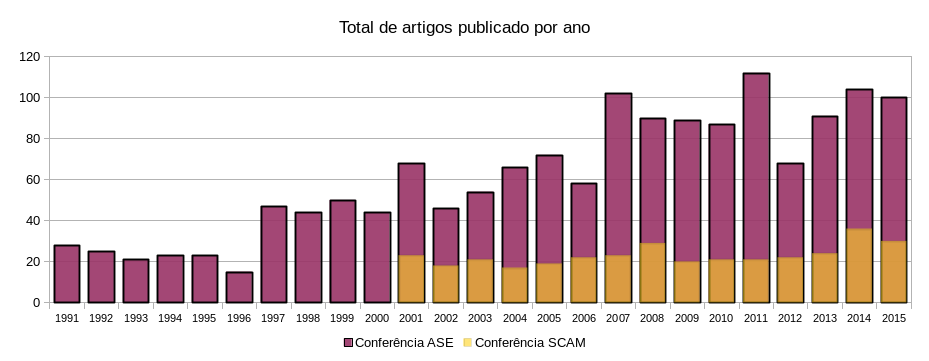
\includegraphics[scale=0.65]{imagens/artigos-por-ano.png}
  \caption{Gráfico em barras com o total de artigos publicado por ano}
  \label{artigos-por-ano}
\end{figure}

\subsubsection{Filtro}

%Dos 346 artigos do SCAM e 1533 artigos do ASE analisados na revisão estruturada
%apenas 44\% (155 artigos) e 18\% (281 artigos) continham os termos pesquisados
%no filtro automático da segunda atividade da revisão, respectivamente.

A segunda etapa filtra o conjunto total de artigos mantendo apenas aqueles que
combinam com os critérios definidos na Tabela \ref{codes-for-filter}, estes
critérios são aplicados de forma automática em cada artigo do conjunto, se um
artigo não satisfaz um ou mais de um destes critérios ele é excluído do
conjunto final.

\begin{table}[h]
\caption{Critérios para filtro de artigos}
\centering
\begin{tabular}{ l l }
  \hline
  Critério                        & String da busca textual               \\
  \hline
  Menciona software acadêmico     & {\tt tool} ou {\tt framework}         \\
  Disponibiliza online            & {\tt download} ou {\tt available}     \\
  Identifica fonte                & {\tt http} ou {\tt ftp}               \\
  Domínio de análise estática     & {\tt static analysis} ou {\tt parser} \\
  \hline
\end{tabular}
\label{codes-for-filter}
\end{table}

O filtro automático percorre os arquivos pdf de cada artigo, aplicando uma
busca textual em todo o conteúdo, incluindo título, resumo, corpo, referências,
apêndices, anexos e demais seções do arquivo. Esta etapa excluiu 1432 artigos
do conjunto inicial, resultando em conjunto, após filtragem, com 441 artigos.

\subsubsection{Seleção}

Na etapa de seleção, os 441 artigos foram lidos com o principal objetivo
de identificar se entre as contribuições do estudo há menção a software
acadêmico de análise estática, identificado minimamente com nome e URL para
obtenção online. 
Essa leitura foi guiada pelos critérios descritos na Tabela \ref{codes-for-selecao}.


Quando a leitura do título, introdução, resultados e conclusão não foi suficiente
para identificar o software utilizamos as demais seções do artigo. Alguns
artigos descrevem a contribuição de software acadêmico em seções específicas,
por exemplo, é comum o uso de notas de rodapé para indicar URL do projeto de
software acadêmico.

Encontramos 62 artigos contribuindo com 60 projetos de software acadêmico de
análise estática. O número de projetos de software é menor do que o número
de artigos porque alguns foram mencionados em mais de um artigo. 
Cada software acadêmico do conjunto foi caracterizado com
as seguintes informações: nome do software, URL do software, título do
artigo, título e ano da confêrencia, como mostra a  Tabela \ref{coding-scheme-software-1}.

\subsection{Caracterização dos projetos selecionados}

As informações coletadas pela seleção de projetos foi complementada por meio de
uma pesquisa manual, em diversas fontes: 
artigo original em que o software foi publicado, site do projeto,
repositório de código fonte, manuais e o próprio código fonte, quando disponível.

As informações descritas na Tabela \ref{coding-scheme-software} foram coletadas 
por meio de inspeção manual no website do projeto, de documentos, manuais e artigos.
Quando o código fonte estava disponível, o código fonte foi explorado em busca de 
informações sobre licença, tipo de entrada e linguagens suportadas.

\begin{table}[h]
\caption{Esquema de características coletadas para cada software acadêmico}
\centering
\begin{tabular}{ l p{11cm} }
  \hline
  Característica           & Explicação \\
  \hline
  Descrição do software    & A descrição do projeto de software \\
  Código fonte disponível  & É possível acessar o código fonte de alguma forma? \\
  Acesso                   & Podemos acessar o software agora? Pode receber os seguintes valores: Sem Acesso, Acesso Pago, Acesso Gratuito \\
  Distribuição             & Como o software é distribuído e pode ser acessado? Pode receber os seguintes valores: gratis, foss, proprietário \\
  Licença                  & O software deixa explícito qual licença é distribuído? \\
%  Permissão para modificar & Os criadores dão permissão para modificar o programa (se não menciona modificação, assume não)?; se permissão apenas por contato, também não \\
  Código fonte             & Em qual linguagem de programação o software acadêmico foi desenvolvido \\
  Entradas suportadas      & Qual o tipo de entrada suportada pelo software de análise estática \\
  Linguagens suportadas    & Quais linguagens de programação o software de análise estática suporta como entrada \\
  \hline
\end{tabular}
\label{coding-scheme-software}
\end{table}

Para identificar a linguagem de programação em que o software foi escrito, utilizamos a
ferramenta livre {\it sloccount}\footnote{http://www.dwheeler.com/sloccount}.

\subsection{Menções ao software}

Após a caracterização de cada software acadêmico, com as informações das Tabelas
\ref{coding-scheme-software-1} e 
\ref{coding-scheme-software}, 
uma revisão da literatura foi realizada nas bibliotecas digitais ACM e IEEE Xplore,
com o objetivo de coletar,
para cada software, as menções na literatura acadêmica ao nome do software.
Um artigo científico pode fazer uma ``menção'' ao software acadêmico 
diversas vezes e de diversas formas -- desde uma simples
menção nos trabalhos relacionados até uma grande contribuição ao software.


Uma string de busca foi definida para cada software acadêmico selecionado.
Além do nome do software pesquisado, as strings de busca incluíram outras
características do software sempre que necessário.
A Tabela \ref{exemplos-strings} apresenta exemplos de strings de busca utilizadas.

\begin{table}[h]
\caption{Exemplos de strings de busca por menções}
\centering
\begin{tabular}{ l p{10cm} }
  \hline
  Nome do software   & String de busca no IEEE Xplore e ACM \\
  \hline
  CodeBoost          & {\tt ((CodeBoost) AND C++)} \\
                     & {\tt content.ftsec:(+CodeBoost +"C++" +Tool)} \\
  \hline
  TestEra            & {\tt (((((TestEra) AND framework) AND Java) AND testing) AND sarfraz)} \\
                     & {\tt content.ftsec:(+TestEra +framework +Java +testing +sarfraz)} \\
  \hline
  XOgastan           & {\tt (XOgastan)} \\
                     & {\tt content.ftsec:(+XOgastan)} \\
  \hline
\end{tabular}
\label{exemplos-strings}
\end{table}

Os resultados foram armazenados localmente em arquivos no formato BibTeX.
Para cada software, os resultados foram agrupados num arquivo único, sem duplicidade
entre os resultados trazidos por cada base bibliográfica. %% Cuidado que ACM cita IEEE.
O arquivo de metadados de cada software contém informações sobre 
o artigo, autores, ano de publicação, conferência, jornal, etc.
Os artigos também foram armazenados localmente, no formato pdf.

Com base nos resultados das buscas, iniciamos a leitura
de cada artigo em busca de confirmar se os autores, de fato, mencionam o
software acadêmico em alguma seção do artigo, e se mencionam, em qual contexto
o software acadêmico é mencionado.

A avaliação dos diversos artigos nos gerou uma escala de tipos de menção ao
software, detalhado na Tabela \ref{coding-scheme-mention}, com 5 valores
distintos, onde o último tipo de menção com maior valor inclui todos os demais.
Um tipo de menção com maior peso inclui implicitamente o tipo de
menção de menor peso, e assim sucessivamente.

\begin{table}[h]
\caption{Tipos de menções ao software acadêmico encontrados nos artigos}
\centering
\begin{tabular}{ l c p{10cm} }
  \hline
  Tipo da menção   & Peso & Explicação \\
  \hline
% * tipo e peso da citação (peso em ordem crescente)
  Não menciona o software  & 0  & Não menciona o nome do software em nenhum contexto \\
  Menciona o software  & 0.1    & Apenas cita o software ou é o mesmo artigo onde o software selecionado; É um artigo com ``mesmo'' conteúdo publicado na ``mesma'' época; O artigo apenas descreve o software; Menciona o software numa tabela com outros, classifica; Menciona o software como exemplo; Menciona o software como trabalho relacionado; Menciona o software em trabalhos futuros \\
  Usa o software   & 0.25    & Avalia ou caracteriza o software; Usa para coleta ou análise de dados; Usa como objeto de estudo; Usa o software como parte de uma solução, implementação, etc; Cria um software derivado mas não disponibiliza as contribuições \\
  Contribui ou integra & 0.5 & Contribuição pequena ou moderada; Extende o software; Integra o software a outros sistemas, formatos de entrada/saída, APIs, etc (seja implementando suporte no software ou do outro lado); Refatora parte do software; Implementa parte do software em outro projeto e compara resultados \\
  Contribui ou cria & 1 & Cria; Contribuição inicial criando o projeto; Faz uma grande contribuição; Refatora todo o software; Abre o código de um software que antes era de código fechado \\
  \hline
\end{tabular}
\label{coding-scheme-mention}
\end{table}

Cada artigo assume, em relação ao software, um valor nesta escala de tipos de
menção. Esta informação foi armazenada no próprio arquivo BibTeX num campo
adicional aos demais campos dos metadados do artigo; ao final, temos os
metadados do artigo como, título, autores, ano de publicação, etc, e 
também o tipo de menção que é feita ao software: se apenas cita como exemplo,
se contribui com novos algoritmos e técnicas, se avalia, ou apenas descreve o
software comparando-o com outro software.

\subsection{Métricas de software}

Ao final, coletamos também algumas métricas do software em relação ao seu
ecossistema de software e em relação a sua qualidade interna: número
total de lançamentos, data e número de versão de cada lançamento, número de
commits e a complexidade estrutural do código fonte.

As informações sobre lançamentos foram coletadas manualmente em arquivos de
changelog, no site do projeto, ou em tags no próprio repositório de código
fonter. O número de commits foi coletado com o uso do git via linha de comando,
o cálculo e coleta da métrica de complexidade estrutural do código fonte foi
coletada com software de análise estática Analizo.
Os dados sobre complexidade estrutural do código fonte não foram utilizados
neste estudo.
% Coloquei a FRASE acima para discutirmos depois.

% \section{Operação} %%%%%%%%
\section{Análise dos Dados} % Raw results from the analysis
\label{sec:study1:analysis}

Dados de 60 projetos de software acadêmico de análise estática desenvolvidos e
publicados na literatura acadêmica de engenharia de software, informações sobre
diversas formas de menção ao nome destes projetos na literatura acadêmica,
o número de autores mencionando o software ao longo do tempo, informações sobre
lançamentos e novas versões do software, atividade de commits no repositório
de código fonte, informaçoes sobre as formas de distribuição e licenciamento,
dados de acesso ao software.

\section{Interpretação dos Resultados} % Hypothesis rejection
\label{sec:study1:interpretation}


\subsection{Q1 - \EstudoDoisQuestaoUm}

% Demográfica.
Todas as trilhas das duas conferências foram incluídas. 
Encontramos 1873 artigos no total, 1527 artigos do ASE e 346
artigos do SCAM, 
com uma média geral de 75 artigos publicados por ano. 

Até o ano de 1996 a conferencia ASE chamava-se KBSE\footnote{ Knowledge-Based
Software Engineering Conference} e só a partir de 1997 mudou para ASE, a
conferência SCAM teve sua primeira edição apenas em 2001, 10 anos após a
primeira edição do ASE.

No geral, a conferência ASE publica quase 4 vezes mais do que a conferência
SCAM, a edição com o maior número de publicações foi 2011 com 112 artigos
publicados, seguido de 2014 com 104, e 2007 com 102, a edição com o menor
número foi 1996 com apenas 15 artigos publicados.

Detalhes sobre o número de artigos
em cada conferência pode ser consultados nos Apêndices
\ref{artigos-do-scam} e \ref{artigos-do-ase} 

%Situação similar ocorreu com o {\it Augmenting
%Counterexample-Guided Abstraction Refinement with Proof Templates} e o {\it
%PtYasm: Software Model Checking with Proof Templates} publicados no ASE 2008,
%fazem referência ao software PtYasm. 
%Por conta disso, entre os 107 artigos, 

%Ainda durante esta última atividade da revisão cada um dos 107 artigos foram
%analisados em busca de informações sobre onde encontrar o software indicado,

Resultou em 60 softwares com indicação de fonte para obtenção do
software, apenas os artigos que indicam endereço de página web para download do
software foram selecionados, ou seja, uma grande parte dos artigos que produzem
softwares acadêmicos nem ao menos citam o software no paper, ou quando citam,
não informam site ou endereço do projeto para download
\cite{allen2017engineering}, seja código fonte ou apenas binários.

... a Figura \ref{softwares-por-ano} apresenta os resultados distribuídos por ano ...

É possível perceber um crescimento no número de software publicados com o
passar dos anos, de forma que podemos confirmar que considerando as
conferências ASE e SCAM, há um crescimento na publicação de softwares
acadêmicos ao longo do tempo.

Apesar da busca na atividade -- (2) Filtro -- utilizar termos com o objetivo de
encontrar apenas softwares disponíveis com informação de onde encontrar o
software, ainda assim, encontramos 45 artigos com publicação de software sem
indicação de fonte para obtenção.

Entre os 1873 artigos, encontramos 107 artigos referenciando 105 softwares de
análise estática, apenas 60 destes indicam a fonte onde o software pode ser
encontrado.

\subsection{Q2 - \EstudoDoisQuestaoDois}

%\citeonline{robles2010replicating} afirma que existe uma tendência das páginas
%web onde os softwares estão disponíveis tem uma grande chance de se tornarem
%indisponíveis ao passar do tempo, investigamos esta tendência 
%cruzando a informação de acesso ao software com a data de publicação do paper
%onde o software foi selecionado.
%a Figura \ref{softwares-disponivel-por-ano} apresenta em cada ano quantos
%porcentos do total de softwares publicados ainda continuam
%disponíveis hoje.

Apenas 37 estão disponíveis, os 23 restantes indicam fonte não mais
acessíveis, endereço não encontrado, indisponível, ou com informações não
relacionadas ao software. 
O Apêndice \ref{resumo-softwares-disponiveis} traz
uma tabela com os nomes e endereços web onde os softwares estão disponíveis.

%Levando em conta a sustentabilidade técnica podemos responder que 
Observamos que 61\% do software acadêmico produzido no domínio de aplicação de análise estática 
são sustentáveis, ou seja, continuam disponíveis ao longo do tempo. 
É importante destacar que não foram considerados aqui artigos que publicaram software 
sem menção à fonte onde o mesmo poderia ser encontrado.
% a revisão estruturada teve como foco encontrar artigos com publicação softwares com indicação de fonte,
% ou seja, aqueles artigos que publicam software mas que não indicam fonte não está sendo
% considerado aqui, vimos que na revisão estruturada, mesmo não sendo o objetivo
Se os artigos que não indicaram a fonte onde o software acadêmico poderia ser encontrado
fossem incluídos -- 45 artigos sem informação de fonte --, 
a taxa de sustentabilidade cairia para apenas 35\%.
Uma revisão estruturada mais abrangente, que desconsiderasse o critério de exclusão
(indicar fonte do software acadêmico), possivelmente resultaria em taxas abaixo dos 35\%, 
sugerindo que a quantidade de software acadêmico publicado em artigos porém indisponível para acesso
pode ser maior do que a encontrada neste estudo.

%TRABALHO FUTURO
%\citeonline{robles2010replicating} afirma que as páginas
%web onde os projetos de software acadêmico foram publicados 
%se tornem indisponíveis com o passar do tempo.
%Podemos investigar esta tendência avaliando os 60 softwares com fonte indicada no artigo,
%identificar se confirmamos neste contexto se com a idade do paper
%as páginas web onde os softwares são publicados tem uma grande chance de se
%tornarem indisponíveis ao passar do tempo.

A Figura \ref{softwares-disponivel-por-ano} apresenta 
um gráfico em linha com o total de projetos de software acadêmico disponíveis por ano.
Também apresenta a porcentagem de software acadêmico publicado com indicação de fonte que ainda estão
disponíveis, ou seja, a taxa de projetos de software que continuam
disponíveis hoje, considerando o conjunto de projetos de software publicado em cada ano 
com informação sobre fonte para download. 
Os anos de 2002, 2004, 2005, e anteriores a 2001 não possuem software publicado
com fonte indicada no artigo ainda disponível e, portanto,
suas informações não aparecem no gráfico.

Ao analisar a Figura \ref{softwares-disponivel-por-ano},
percebemos que há um leve crescimento na disponibilidade
dos projetos de software acadêmico  nos anos mais recentes.
%
Existe uma leve tendência, ao longo dos anos,  
para a indisponibilidade das fontes informadas e páginas web.
É possível notar que, em 2006, 80\% de todos os
softwares de análise estática publicados nas conferências ASE e SCAM ainda estão disponíveis.
Este número cresce em 2014, chegando a 90\%, e cai no ano seguinte para 85\%.
Apesar de não estar sempre crescente, e da  amostra pequena usada neste estudo 
-- apenas 60 projetos de software acadêmico,
este leve indício confirma a afirmação de \citeonline{robles2010replicating}.

Os 37 softwares com fonte disponível foram avaliados em relação ao segundo
aspecto, isto é, com respeito à forma em que estão disponíveis:
se os artigos informam onde obter tais softwares, se os softwares estão realmente disponíveis, e 
se, ao acessar as fontes indicadas na presente data deste estudo, os softwares estão funcionando e
acessíveis.

Do conjunto de 37 projetos de software estudados, %% Joenio, coloquei aqui o tempo no PRETERITO -- revisar outras partes.
3 não disponibilizaram seu código fonte e  %% Joenio, mudei as frases para VOZ ativa, sujeito: projeto de software.
34 disponibilizaram o código fonte publicamente.
Dentre os que disponibilizaram o código fonte, 13 não informaram licença alguma
%apesar de ter o código fonte disponível, 
e 21 informaram licenças de FOSS ({\it free and open source software}):

\begin{itemize}
  \item 8 usam GNU General Public License;
  \item 2 usam Apache License;
  \item 4 usam BSD License;
  \item 3 usam Eclipse Public License;
  \item 2 usam University of Illinois/NCSA Open Source License;
  \item 1 usa licença {\it FrontEndART Software Ltd}; e
  \item 1 usa licença {\it SAnToS Laboratory Open Academic License}.
\end{itemize}

Entre os 37 softwares disponíveis, 21 podem ser modificados para se adaptar às
necessidades emergentes sem necessidades de solicitação prévia de autorização
aos autores originais devido ao uso de licenças livres. 
Os 13 softwares restantes com código fonte disponível mas sem licença expressa podem
ser modificados, mas a falta de uma licença impõe a necessidade
de solicitar permissão aos autores originais.

35\% dos softwares disponíveis podem ser adaptados de forma incremental para
aproveitar oportunidades emergentes, 21\% podem mediante prévia autorização do
autor original serem modificados, e apenas 5\% não oferecem essa possibilidade
por não disponibilizarem o código fonte publicamente.

%4º Princípio, Persistencia.    % ??????

Os identificadores únicos e metadados descrevendo o software e sua disposição
devem persistir - mesmo além do tempo do software que descrevem.

%Deste total apenas 11\% (41 artigos) e 4\% (62 artigos) foram selecionados na
%terceira e última atividade da revisão contendo publicação de ferramenta de
%análise estática.

%Resultando em 103 artigos com publicação de {\it software científico} de
%análise estática de código fonte, apenas 35 possuem fonte para obtenção do
%software, sendo 32 de código aberto, ou seja, com disponibilidade de
%código fonte, e 3 grátis, apenas binários disponível. Ou seja, apenas 31\% dos
%artigos com publicação de software disponibilizam o código fonte das mesmas.
%Isto significa que 69\% dos artigos com publicação de software de análise
%estática de código fonte são potencialmente impossíveis de serem repetidos, já
%que os artefatos originais são necessários para tal atividade e o artigo não
%disponibiliza o código fonte dos mesmos.

\subsection{Q3 - \EstudoDoisQuestaoTres}

Número de menções a cada software acadêmico e qual o contexto e tipo de menção
é feita, quem e quantos são os autores de cada menção.

...

%cada citação pontua no máximo 1 ponto para o peso final do paper ao quanto
%contribui para a sustentabilidade técnica do software, esta pontuação será
%calculada com base nos pesos (em porcentagem) 'contribution\_weight' e
%'authorship\_weight', este último valor é aplicado à contribution weight,
%ou seja contribution\_weight é acrescido a partir do valor de authorship\_weight.
%o valor final se ultrapassar 1 será cortado no limite 1 (máximo), a ideia não é muito
%os números, não queremos saber se são numeros altos, queremos constancia, queremos
%medir se existe um nível de contribuição mínimo aos softwares, isto está
%sendo proposto como algo que mantém o software vivo e útil para a comunidade
%acadêmmica. (por hora o valor mínimo "ideal" por ano é "0.5", ou seja, um
%valor bem modesto, este valor indica que houve ao menos uma contribuição
%ao software, ou que teve citações suficientes equivalente a uma contribuição,
%o software ao ser muito citado ganha mais visibilidade, impacta na possibilidade
%de maior adoção e maior contribuição por terceiros.

\subsection{Q4 - \EstudoDoisQuestaoQuatro}

Os dados coletados sobre as menções a cada software foram acrescentados com uma
nova informação calculada a partir da autoria de cada artigo mencionando o
software, representado numa escala de peso quantos novos atores foram incluídos
no ecossistema daquele software, isto foi feito comparando o conjunto de autores
da publicaçao com o conjunto acumulado de todos os autores anteriores, 
podendo assumir um dos valores da Tabela \ref{coding-scheme-author}.

%segundo a publicação
%representa

\begin{table}[h]
\caption{Autoria das menções ao software acadêmico encontradas nos artigos}
\centering
\begin{tabular}{ l c p{10cm} }
  \hline
  Novos atores no ecossistema & Peso & Explicação \\
  \hline
  Criadores & 0 & São os primeiros autores a publicar sobre o software \\
  Nenhum    & 0.1 & Todos os autores já publicaram sobre o software em anos anteriores \\
  Parte     & 0.25 & Uma parte dos autores já publicou sobre o software em anos anteriores \\
  Todos     & 0.5 & Nenhum dos autores jamais publicou sobre o software \\
  \hline
\end{tabular}
\label{coding-scheme-author}
\end{table}

A comparação entre os nomes do autores passou antes pela normalização
no formato de representação, visto que cada artigo utiliza um formato
de nome diferente, transformamos, por exemplo, ``Bajaj, Kon'' em ``Bajaj K.'',
``Costa, Kim A.'' em ``Costa K. A.'', ``Rajan, Sreeranga P.'' em ``Rajan S. P.'',
``Pol, Jaco van de'' em ``Pol J. van de'', ``Zijiang Yang'' em ``Yang Z.'',
e assim comparamos dois nomes considerando que cada um destes nomes representa,
de forma única, um autor.

Acesso ao software

5º Princípio da citação ao softwares, Acessibilidade:

``citações aos softwares devem permitir e facilitar acesso ao software,
metadados, documentação, dados e outros materiais necessários tanto
para humanos quanto para máquinas se informar do referido software''

Não significa que o software deva estar disponível gratuitamente, mas que
os metadados devem prover informação suficiente para que o software seja
acessado. Se o software é livre, os metadados devem prover um identificador
que pode ser resolvido para uma URL apontando para a versão específica
do software sendo citado.

Pra softwares comerciais, os metadados devem ainda prover informações sobre
como acessa o software, mas pode ser um número de telefone da empresa que
vende o software ou o link para um site que venda o software

\cite{smith2016software}

5. Accessibility: Software citations should facilitate access to the software itself and to its

%outro fator de peso para definir o valor final do peso é se houve lençamentos
%de novas versões do software naquele ano, se houve ao menos 1 versão lançada,
%isso leva o final\_weight para o valor máximo 1.0 (que representa 100\%)

\subsection{Ameaças à validade}

Validade de construção.
A leitura dos artigos na revisão estruturada para identificar se publicam
softwares de análise estática de código fonte, se disponibilizam fonte para
obtenção de tais softwares, e se os softwares são mesmo do domínio de aplicação
de análise estática de código fonte podem ter maior validade se feitos em
par e revisados por outros pesquisadores.
Neste estudo, estas atividades foram realizadas pelo autor desta dissertação e 
não houve revisão por pesquisadores independentes.
%% A ameaça não foi tratada.

Validade externa. Apenas duas conferências. Apenas duas bases. Apenas um domínio de software acadêmico / uma área do conhecimento em que pesquisadores também programam.
%% A ameaça não foi tratada.

\section{Conclusões}

FALTA uma síntese aqui. 
Este estudo ...
Resultados mostram que ...
Algumas tendências emergiram a partir da leitura ...

Planejamos fazer outro estudo ... 

Todas as atividades e artefatos produzidos neste estudo estão documentados em
repositório público no
Github\footnote{\url{http://github.com/joenio/dissertacao-ufba-2016}}, o
Apêndice \ref{apendice-revisao-estruturada} traz mais informações.

%%%%%%%%%%%%%%%%%%%%%%%%%%%%%%%%%%%%%%%%%%%%%%%%%%%%%%%%%%%%%%%%%%%

%, uma lista completa e
%o endereço de cada edição onde os artigos foram obtidos está documentado no
%Apêndice \ref{edicoes-conferencias}

%% usar a dimensao abaixo para definir quais usar na avaliacao longitudinal:
%% 
%% %, e qual a frequência de lançamentos indicando se são
%% %atualizadas frequentemente ou estão obsoletas.
%% 
%% \begin{description}
%% 
%%   \item {\it Lançamentos ({\it Releases}) - quantos lançamentos por ano:}
%%     \begin{itemize}
%%       \item Frequentemente $>=$ 3 vezes ao ano\\
%%         {\it \small novas versões da ferramenta são lançadas 3 ou mais vezes por ano}
%%       \item Ocasionalmente $<$ 3 vezes ao ano\\
%%         {\it \small novas versões da ferramenta são lançadas menos que 3 vezes ao ano}
%%       \item Obsoleta 0 vezes ao ano\\
%%         {\it \small intervalo entre novos lançamentos é maior que 1 ano}
%%     \end{itemize}
%% 
%% \end{description}
%% 
%% O autor não deixa claro como categorizar softwares sem lançamentos nos últimos
%% anos mas com histórico de lançamento frequente em anos anteriores. Assim, será
%% considerado todo o histórico de lançamentos e só serão considerados obsoletos
%% por exemplo softwares que nunca tenha tido mais de 1 lançamento ao ano
%% considerando todo o histórico dele. Da mesma forma, será considerado ocasional
%% apenas aqueles que sempre tiveram no máximo 2 lançamentos ao ano. Esta dimensão
%% irá nos dizer o grau de evolução de cada ferramenta, considerando que softwares
%% com lançamentos frequentes estão evoluindo.
%% 
%% ======================
%% 
%% \begin{description}
%% 
%%   \item {\it Entrada - quais tipos de arquivos podem ser carregados na ferramenta:}
%%     \begin{itemize}
%%       \item Código-fonte - arquivos de código texto podem ser carregados
%%       \item Byte code - arquivos com Java Byte Code ou Microsoft
%%       \item Linguagem intermediária (MSIL) pode ser carregada
%%     \end{itemize}
%% 
%%   \item {\it Linguagens suportadas - quais linguagens de programação a ferramenta suporta:}
%%     \begin{itemize}
%%       \item .NET - todas as linguagens compiladas em bibliotecas ou programas no framework .NET
%%       \item VB .NET - suporta VB.NET
%%       \item C\# - suporta C\#
%%       \item Java - suporta linguagem de programação Java
%%       \item C, C++ - suporta linguagem de programação C ou C++
%%     \end{itemize}
%% 
%% \end{description}
%% 
%% As dimensões apresentada por \citeonline{Novak2010} não cobrem alguns aspectos
%% importantes percebidos ao longo deste estudo, assim novas dimensões serão utilizadas
%% em complemento às dimensões citadas acima.
%% 
%% \begin{description}
%% 
%%   \item {\it Linguagem de programação - em que linguagem de programação à ferramenta é escrita:}
%%     \begin{itemize}
%%       \item .NET
%%       \item VB .NET
%%       \item C\#
%%       \item Java
%%       \item C, C++
%%     \end{itemize}
%% 
%% \end{description}
%% 
%% \subsection{Ferramentas da indústria}
%% 
%% Em paralelo à revisão estruturada para seleção de ferramentas da academia
%% foi realizada uma seleção manual no catálogo de ferramentas de análise estática do projeto
%% SAMATE\footnote{https://samate.nist.gov/index.php/Source\_Code\_Security\_Analyzers.html}
%% em busca de ferramentas da indústria.
%% 
%% O projeto SAMATE\footnote{http://samate.nist.gov} - {\em Software Assurance
%% Metrics and Tool Evaluation}, um projeto do NIST\footnote{http://nist.gov}
%% dedicado ao desenvolvimento de métodos que permitam avaliar e medir a
%% eficiência de ferramentas e técnicas sobre garantia de qualidade em software.
%% O site do projeto, disponível em \citeonline{SamateAnalysers}, mantém uma lista
%% de ferramentas de análise estática.
%% 
%% Nesta busca por ferramentas da indústria encontramos um total de 54 ferramentas
%% presentes no catálogo do projeto SAMATE, 19 tinham código-fonte disponível,
%% destas apenas 14 eram suportadas pelo Analizo (escritas em C, C++ ou Java).
%% 
%% Após download do código-fonte de cada ferramenta selecionada, em sua versão
%% mais recente, a ferramenta Analizo será utilizada para a coleta das métricas. 
%% A Tabela \ref{total-de-ferramentas} traz um resum com todas as ferramentas
%% selecionadas, tando da indústria quanto da academia.
%% 
%% Deste total de 35, 4 tem lançamentos frequentes, 9 são obsoletas, 8 tem
%% lançamentos ocasional e 14 não possui informação sobre lançamentos.
%% 
%% Uma vez identificados os artigos que publicaram ferramentas do domínio
%% desejado, procuramos no próprio artigo por referências de onde encontrar o
%% código-fonte da ferramenta. Neste momento, pode-se enfrentar algumas situações.
%% 
%% \begin{itemize}
%% 
%%   \item Os autores afirmam que a ferramenta está disponível mas o artigo
%%     não contém referências de onde encontrar o código-fonte, estes
%%     autores serão contactados, por email, solicitando informações de onde
%%     obter o código-fonte da ferramenta.
%% 
%%   \item O artigo indica onde obter o código-fonte da ferramenta, mas o acesso ao local
%%     indicado não está disponível, ou está disponível mas o software não se
%%     encontra lá, os autores serão contactados, solicitando informações
%%     atualizadas de onde obter uma cópia do código-fonte da ferramenta.
%% 
%%   \item Artigos que indicam onde obter o código-fonte da ferramenta e a referência
%%     está correta. Será feito o download do código-fonte da última versão
%%     disponível.
%% 
%% \end{itemize}
%% 
%% Uma vez que os autores sejam contactados por email e respondam com informações
%% sobre onde obter o software, a ferramenta é adicionada ao conjunto de
%% ferramentas a serem analisadas.
%% 
%% \begin{description}
%% 
%%   \item {\it Contexto - onde a ferramenta surgiu:}
%%     \begin{itemize}
%%       \item Academia - foi desenvolvida inicialmente em contexto acadêmico
%%       \item Indústria - foi desenvolvido fora da academia
%%     \end{itemize}
%% 
%%   \item {\it Tamanho em número de classes - número de classes/módulos da ferramenta}
%% 
%%   \item {\it Nível de manutenabilidade - interpretação das seguintes métricas de código-fonte:}
%%     \begin{itemize}
%%       \item Complexidade Estrutural
%%       \item Custo de Mudança
%%     \end{itemize}
%% 
%% \end{description}

%\section{Avaliação da sustentabilidade técnica}
%\label{sustentabilidade-tecnica}

%apesar disso, antes mesmo de resolver tais questões é
%fundamental compreender os impactos que eles causam na comunidade de pesquisa.

%, dados sobre cada software acadêmico e
%informações sobre o seu ecossistema.

%A Tabela \ref{coding-scheme-mentions} descreve as informações
%coletadas para cada projeto.

%\begin{table}[h]
%\caption{Esquema de codificação para menções a software acadêmico como contribuição}
%\centering
%\begin{tabular}{ l p{10cm} }
%  \hline
%  Código                   & Definição \\
%  \hline
%  Nome do software         & O nome do projeto de software \\
%  URL                      & Endereço web do software ou projeto, site ou repositório de código fonte, com o software disponível \\
%  Título do artigo         & Título do artigo onde o software é citado como contribuição, seja principal ou secundária \\
%  Nome do evento           & Nome da conferência onde o software foi publicado \\
%  Ano do evento            & Ano da edição da conferência onde o artigo foi publicado \\
%  \hline
%\end{tabular}
%\label{coding-scheme-mentions}
%\end{table}

%Este esquema de codificação foi inspirado no {\it Coding scheme for mentions of
%software} proposto no trabalho de \citeonline{howison2016software}.

%O conjunto estudado representa um corte transversal nas publicações de dois
%eventos tradicionais da engenharia de software, análise estática, uma área com
%um bom histórico ...

%identificará os possíveis falsos negativos deste conjunto reduzido deixando-os
%fora do resultado final.

%Cada critério são aplicados de forma automática numa busca textual aplicada
%em todo o conteúdo de cada artigo selecionado na etapa anterior, a string de
%busca final tem o objetivo geral de ser abrangente a fim de evitar falsos
%negativos, ou seja, evitar que o filtro deixe de fora artigos que publiquem
%software de análise estática.

%é esperado encontrar resultados com
%falso positivo, ou seja, artigos com publicação de software acadêmico de outros
%domínios, ou artigos com publicação de software acadêmico mas sem menção
%à fonte online para obtenção, entre outras situações.

%cada um destes projetos foram devidamente identificados
%com nome e URL, e estão disponíveis para download segundo os autores.

%Dois dos resultados de software acadêmico
%encontrados são mencionados em dois artigos, resultado ao final 60 projetos de
%software acadêmico, 

%Software
%acadêmico que seja mais abrangente do que apenas análise estática de
%código fonte mas que contenham esta função em seu conjunto também são
%selecionados.

%O objetivo foi conseguir caracterizar cada software com todas
%as 
%Os softwares disponíveis foram avaliados em relação à disponibilidade de código
%fonte e à licença utilizada, essas informações, ...

%se os autores mencionam alguma contribuição
%ao software, ou se o software foi utilizado apenas para coleta de dados, ou se
%nem mesmo mencionam o nome do software.

%a busca por ocorrências ao nome do
%software foi realizado com o auxílio da funcionalidade de busca do leitor de
%pdf utilizado para ...
%mecanismo de busca do leitor de
%pdf\footnote{Utilizamos o software livre Evince versão 3.22.1} utilizado para
%leitura dos artigos, com o auxílio da busca encontramos cada ocorrência ao nome
%do software tomando nota sobre o contexto e o uso que é feito do software neste
%contexto

%foi lido em busca de encontrar menções ao nome do software,
%em qual contexto o software é mencionado e de que forma é mencionado,
%a Tabela \ref{coding-scheme-mention} resume cada
%tipo de menção com explicação dos casos em que se enquadram,
%o método utilizado
%para .

%das bibliotecas digitais, temos para cada um dos artigos todos os seus
%metadados,. Os autores de
%cada uma das menções ao software, por exemplo, serão utilizados na fase de
%análise para calcular o quanto de autores novos começaram a publicar sobre
%certo software acadêmico.

%Quanto ...  Na literatura científica publicada nas conferências ASE e SCAM ...
%do ponto de vista da literatura acadêmica e do seu ecossistema de software acadêmico:
%O que a literatura acadêmica publicada nos diz sobre os projetos de software
%acadêmico publicados nas conferências ASE e SCAM?
%Podemos adaptar de forma incremental os softwares acadêmicos de análise estática para aproveitar oportunidades emergentes, sem perda de reprodutibilidade?

% o artigo com resumo do RESER 2011 diz \cite{knutson2010report}:
% 4) Re-
% search tools are either not available or not usable, so precise
% replication is impractical [1, 2, 8, 18, 19].

%e possui uma média de 23 artigos publicados por edição.
%com uma média geral de 75 artigos publicados por ano. 
%Neste período a conferência ASE teve uma média de 80 artigos
%publicados por ano, se for levado em conta todas as edições, apenas da
%conferência ASE, a média cai para 61 artigos por ano.

%(2) Filtro -- reduziu em 77\%
%o número total de artigos, resultando em ??? (metodologia) artigos
%para serem analisados na próxima etapa da revisão estruturada.  Durante a execução desta
%atividade foi necessário analisar dois artigos manualmente, {\it Adaptable
%concern-based framework specialization in UML} e {\it Property-oriented test
%generation from UML Statecharts}. O conteúdo destes dois artigos não é possível
%de ser analisados pelo script de filtro uma vez que é formado por imagens
%digitalizadas, ambos artigos publicados no ASE edição 2004. Nenhum dos dois
%artigos continham os termos pesquisados e ficaram fora do conjunto selecionado
%nesta atividade.

%alguns destes
%artigos fazem referência à um mesmo software, é o caso do {\it BEST: A symbolic
%testing tool for predicting multi-threaded program failures} e do {\it Scalable
%and precise symbolic analysis for atomicity violations}, ambos publicados no
%ASE 2011 fazem referência ao software BEST.

%em cima dos 441 artigos selecionou 107 artigos com publicação de software
%acadêmico, temos 105 softwares distintos, uma lista com todos os softwares e
%uma breve descrição de cada um é apresentado no Apêndice
%\ref{resumo-softwares}, 

%Apesar da busca na atividade -- (2) Filtro -- utilizar termos com o objetivo de
%encontrar apenas softwares disponíveis com informação de onde encontrar o
%software, ainda assim, encontramos 45 artigos com publicação de software sem
%indicação de fonte para obtenção.

%Entre os 1873 artigos, encontramos 107 artigos referenciando 105 softwares de
%análise estática, apenas 60 destes indicam fonte onde o software pode ser
%encontrado.

%identificar se confirmamos neste contexto se com a idade do paper
%as páginas web onde os softwares são publicados tem uma grande chance de se
%tornarem indisponíveis ao passar do tempo.

%A Figura \ref{softwares-disponivel-por-ano} apresenta em cada ano quantos
%porcentos do total de softwares publicados com indicação de fonte estão ainda continuam
%disponíveis hoje, ou seja, quantos qual é a taxa de softwares que continuam
%disponíveis hoje dentro do conjunto de softwares publicados em cada ano com
%informação sobre fonte para download.  Os anos de 2002, 2004, 2005, e
%anteriores a 2001 não possuem softwares publicados com fonte indicada no artigo
%ainda disponível, portanto não constam no gráfico suas informações.

%O Apêndice \ref{resumo-softwares-disponiveis} traz
%uma tabela com os nomes e endereços web onde os softwares estão disponíveis.

%Levando em conta a sustentabilidade técnica podemos responder que 61\% dos
%softwares produzidos no domínio de aplicação de análise estática são
%sustentáveis, ou seja, continuam disponíveis ao longo do tempo. Lembrando que
%não está sendo considerado aqui pesquisas que publicam software sem menção à
%fonte onde pode ser encontrado o software, a revisão estruturada teve como foco encontrar
%artigos com publicação softwares com indicação de fonte, ou seja, aqueles
%artigos que publicam software mas que não indicam fonte não está sendo
%considerado aqui, vimos que na revisão estruturada, mesmo não sendo o objetivo
%encontramos 45 artigos sem informação de fonte, isto faria esta taxa cair para
%apenas 35\%, uma revisão estruturada mais abrangente com objetivo de encontrar
%todo e qualquer software, independente de indicar fonte ou não, com certeza
%faria esta taxa cair abaixo dos 35\%, indicando que o número de softwares
%publicados e hoje indisponíveis é maior que os números encontrados neste estudo.

%4º Princípio, Persistencia
%
%Os identificadores únicos e metadados descrevendo o software e sua disposição
%devem persistir - mesmo além do tempo do software que descrevem.

%Deste total apenas 11\% (41 artigos) e 4\% (62 artigos) foram selecionados na
%terceira e última atividade da revisão contendo publicação de ferramenta de
%análise estática.

%Resultando em 103 artigos com publicação de {\it software científico} de
%análise estática de código fonte, apenas 35 possuem fonte para obtenção do
%software, sendo 32 de código aberto, ou seja, com disponibilidade de
%código fonte, e 3 grátis, apenas binários disponível. Ou seja, apenas 31\% dos
%artigos com publicação de software disponibilizam o código fonte das mesmas.
%Isto significa que 69\% dos artigos com publicação de software de análise
%estática de código fonte são potencialmente impossíveis de serem repetidos, já
%que os artefatos originais são necessários para tal atividade e o artigo não
%disponibiliza o código fonte dos mesmos.
